 \documentclass[11pt]{article}

\usepackage{latexsym}
\usepackage{amssymb}
\usepackage{amsthm}
\usepackage{amscd}
\usepackage{amsmath}
\usepackage{tikz}
\usepackage{graphicx}
\usepackage{enumerate}

\newcommand{\ZZ}{\mathbb{Z}}

\setlength{\evensidemargin}{1in}
\addtolength{\evensidemargin}{-1in}
\setlength{\oddsidemargin}{1.5in}
\addtolength{\oddsidemargin}{-1.5in}
\setlength{\topmargin}{1in}
\addtolength{\topmargin}{-1.5in}

\setlength{\textwidth}{16cm}
\setlength{\textheight}{23cm}

\newcommand{\rook}{\hspace{-.1cm}\amalg\hspace{-.15cm}\bar{}}
\newcommand{\Stab}{\mathrm{Stab}}
\newcommand{\FF}{\mathbb{F}}


\begin{document}
\begin{center}
\section*{William Daniels}
\section*{CSCI 4202}
\subsection*{Artificial Intelligence}
\subsection*{Homework \#3 02/15/15}
\end{center}

\vspace{.25cm}
\begin{enumerate}
\item Construct heuristic function and apply an $A^*$ algorithm to the problem "Missionaries and Cannibals".\\\\
\textbf{Solution:}\\\\
First, we establish our state space: 
state space $(c, m)$:
\begin{align*}
&c\text{ is the number of cannibals on side B of the river}\\
&m \text{ is the number of cannibals on side B of the river}\\
\end{align*}
Now, the heuristic function for this problem is determined as follows: For each missionary on the 'B' side of the river, add 1, for each missionary on the 'A' side of the river, subtract one. For each cannibal on side 'B' of the river, add 1, and for each cannibal on side 'A' of the river, subtract 1. If there are more cannibals than missionaries on either side of the river, subtract 1 for each cannibal above the number of missionaries on each side of the river. If there are no missionaries on a side, don't add anything. If the number of missionaries and cannibals on both sides of the river is the same, add 1. \\\\
You can see the A* search below. The open/closed list looks like the following: 
\begin{enumerate}
\item open-list: [S1]\\
closed-list: []
\item open-list: [S2, S5, S10]\\
closed-list: []
\item open-list: [S5]\\
closed-list: [S2, S10]
\item open-list: [S12, S11, S5]\\
closed-list: [S2, S10]
\item open-list: [S1, S5, S12, S11]\\
closed-list: [ S2,S10]
\item open-list: [S1, S5, S12]\\
closed-list: [S2, S10, S11]
\item open-list: [S1, S5, S12, S7]\\
closed-list: [S2, S10, S11]
\item open-list: [S1, S5, S12, S7, S8]\\
closed-list: [S2, S10, S11]
\item open-list: [S1, S5, S12, S7, S8, S15]\\
closed-list: [S2, S10, S11]
\end{enumerate}


\begin{figure}[ht!]
\centering
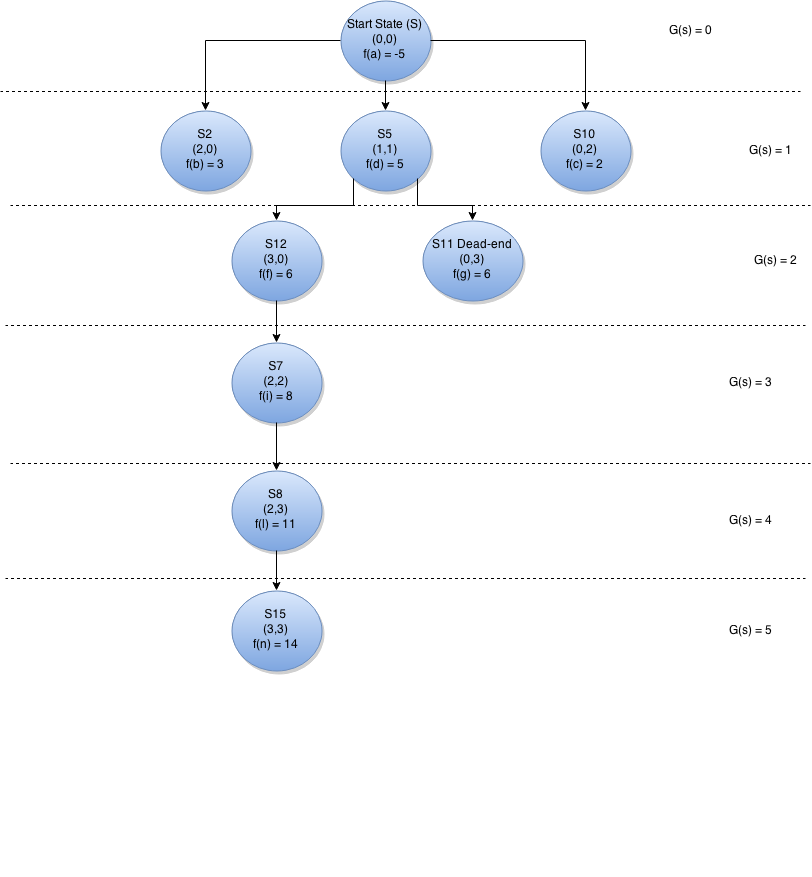
\includegraphics[width=110mm]{HW3StateDiagram.png}
\caption{State Diagram and A* search for Missionaries and Cannibals problem \label{overflow}}
\end{figure}
Note that the search is massively simplified due to the heuristic being pretty accurate, not to mention the 'allowed legal moves' where we don't have cannibals overtaking (eating) the missionaries creates only a few states once we're upon the proper path in the beginning. So really the only choice state is the first one. 


\item Use the following heuristic function $E(n)$ and apply Algorithm MINIMAX (With Alpha-Beta cut-offs) with limited depth to the game tic-tac-toe. Pick 3 different position of this game as start states and show 2-ply and 3-ply searches for each of them. Compare results of the 2-ply and 3-ply searches for the same states. Explain. You have to show 6 (= 3 X2) different searches totall. Show cut offs. (dont take start positions considered in class. Don't apply unlimited depth search.). \\\\

See attached scanned-image. Sorry for the scan, but it was too difficult to get this into digital form purely. Maybe next time. 
\begin{figure}[ht!]
\centering
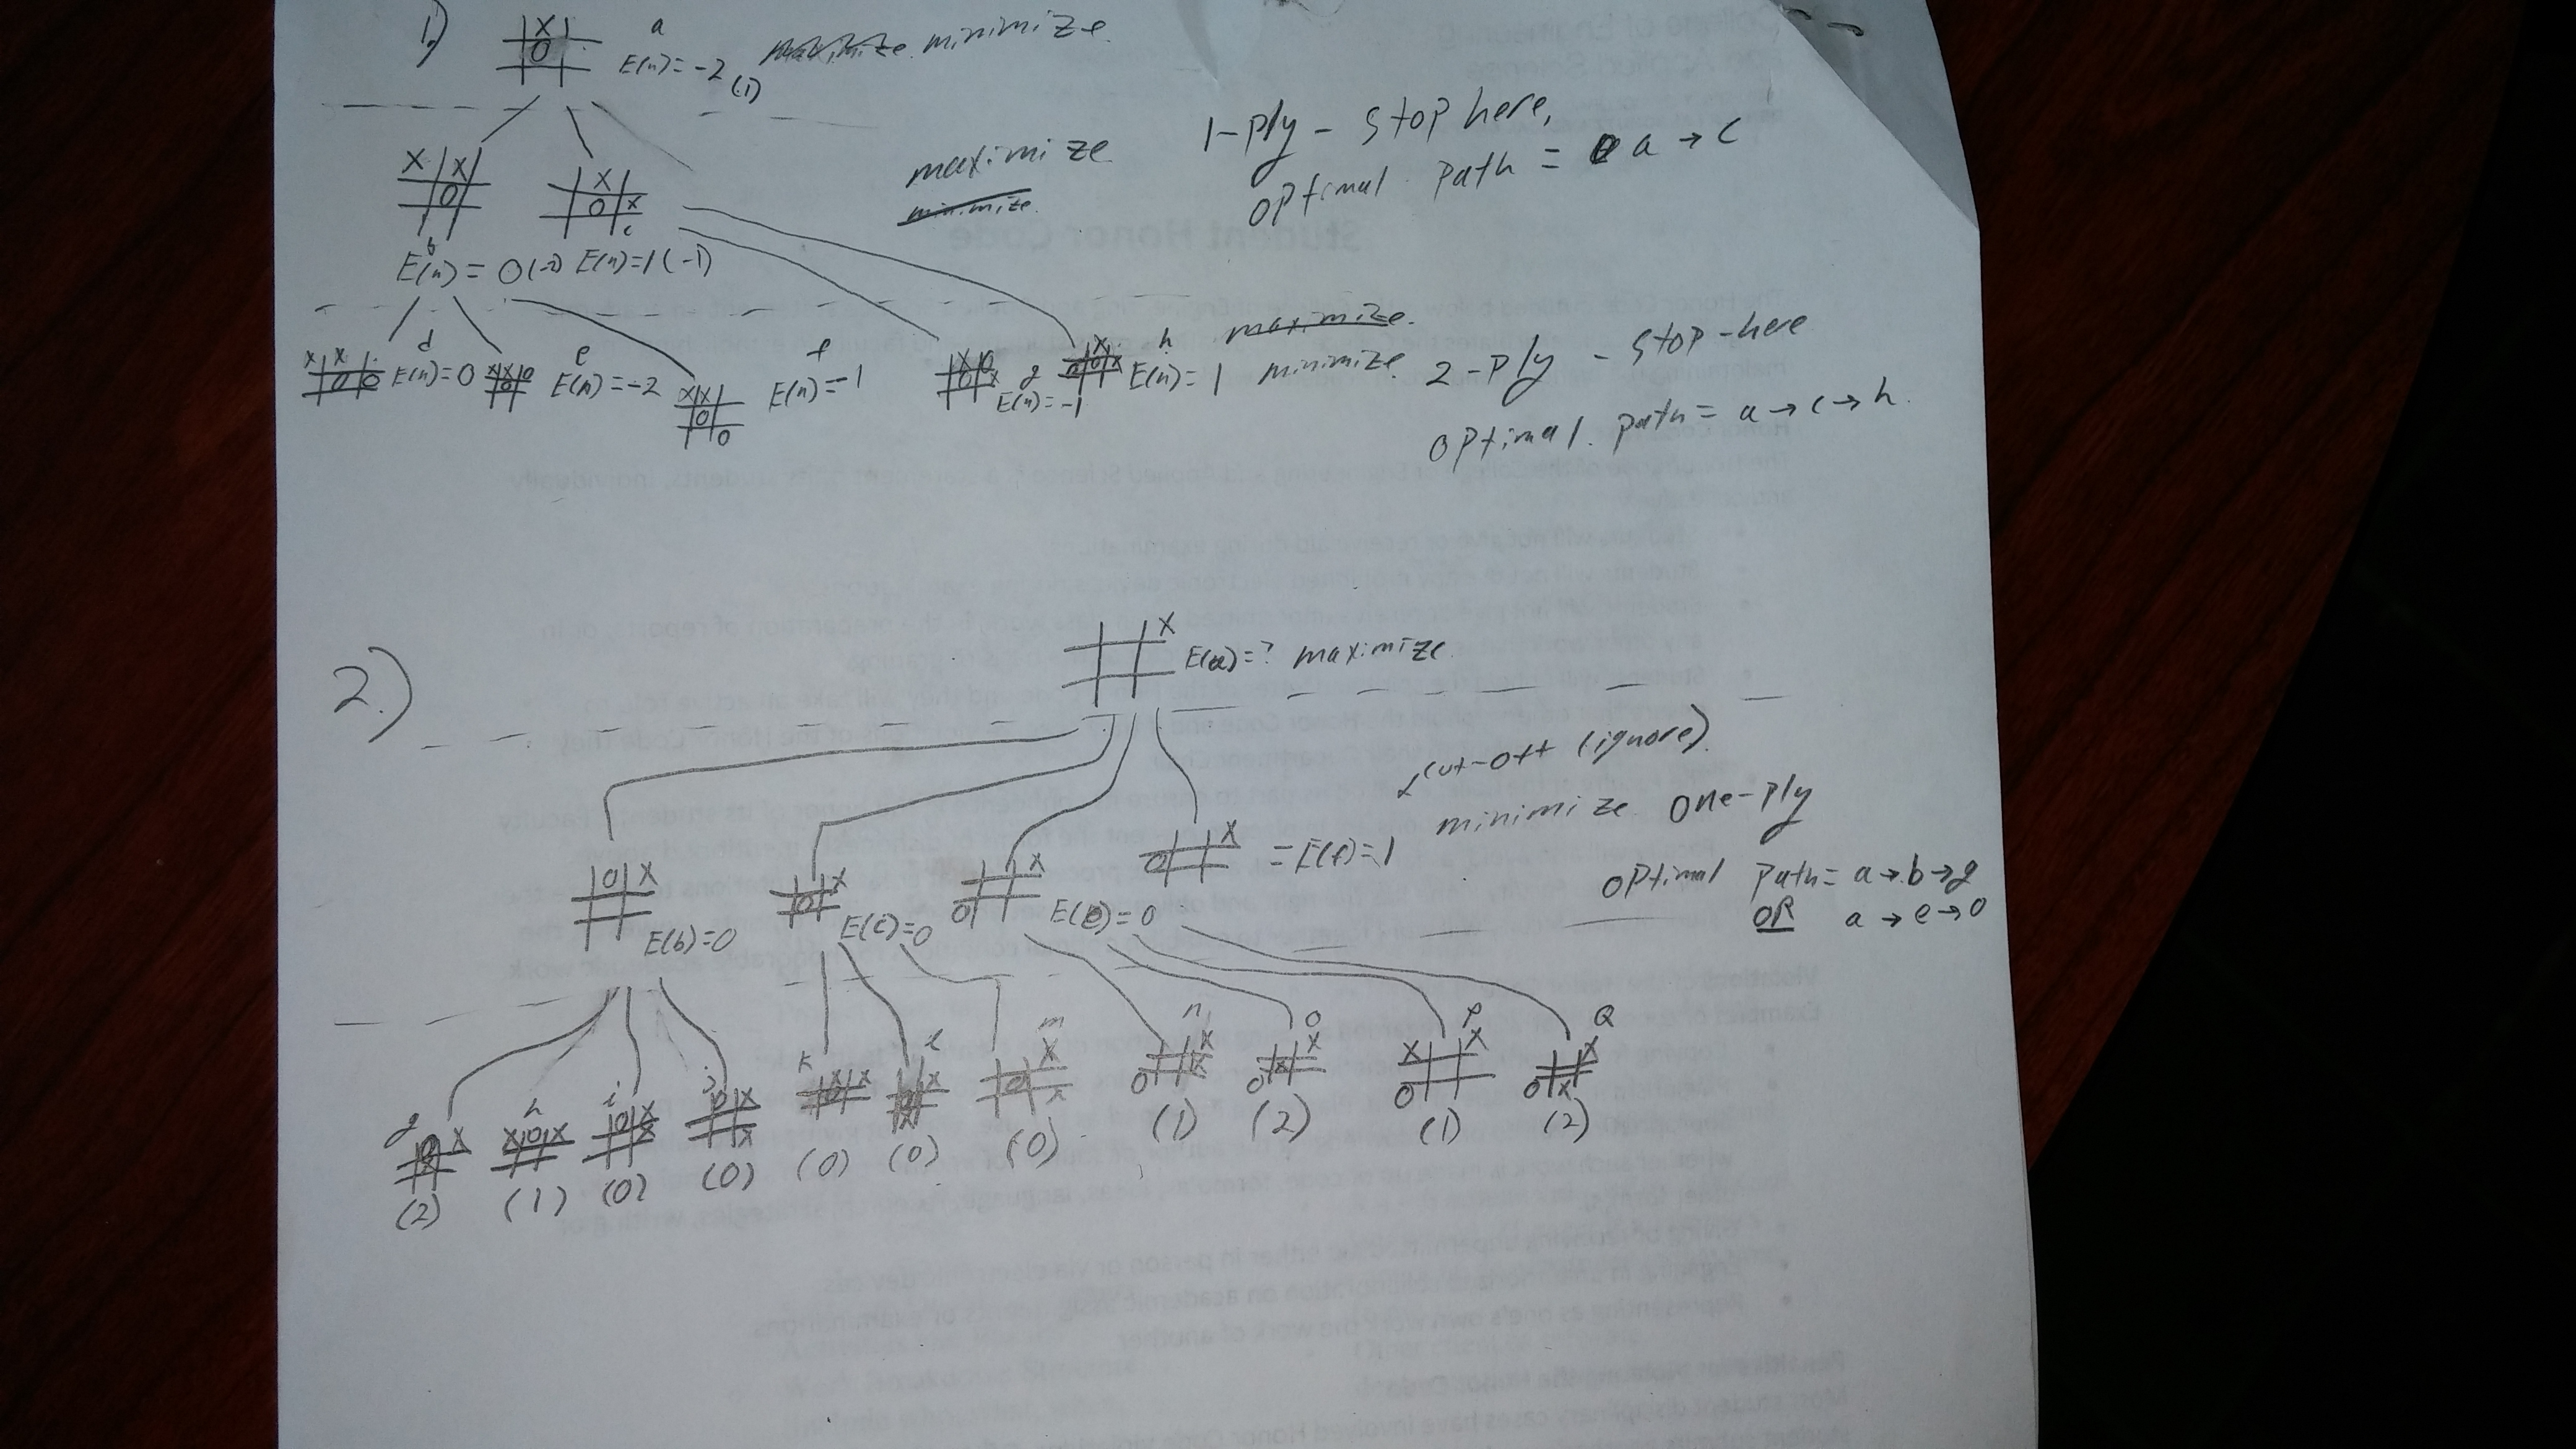
\includegraphics[width=200mm]{HW3MINIMAXAI.jpg}
\caption{minimax search 1 and 2-ply for tic-tac-toe \label{overflow}}
\end{figure}
\end{enumerate}





\end{document}

